\documentclass[a4paper,10pt]{article}
\usepackage[utf8]{inputenc}
\usepackage{graphicx}
\usepackage{hyperref}
\usepackage{dirtree}
\usepackage{listings}
\graphicspath{/mnt/data_1/code/asignaturas/sint/practicas/pr2}
\newcommand\tab[1][1cm]{\hspace*{#1}}
\title{Técnicas de Búsqueda Heurística (3ª semana)}
\begin{document}
\maketitle
\pagebreak
\section{Ejercicio 1}
\subsection{Enunciado}
Sea el siguiente grafo, en el que los arcos tienen un coste y los nodos una estimación
heurística de su distancia al nodo Z (Z es el nodo objetivo y A es el nodo inicial).
\begin{enumerate}
	\item Sin ningún conocimiento a priori (sin conocer la estructura del grafo, sus pesos...) ¿qué podrías hacer para asegurarte de que A* encuentra el camino mínimo hasta el nodo solución?
	\item Observando el grafo, pero sin aplicar A* ¿puedes asegurar si este método encontrará o no el camino mínimo entre A y Z?
	\item Aplica el algoritmo A*. Dibuja en cada etapa del algoritmo el subgrafo parcial creado y la situación de las listas ABIERTA Y CERRADA.
\end{enumerate}
\subsection{resolución}
\subsubsection{Sin ningún conocimiento a priori (sin conocer la estructura del grafo, sus pesos...) ¿qué podrías hacer para asegurarte de que A* encuentra el camino mínimo hasta el nodo solución?}
Si se aplica la busqueda por profundidad iterativa, la busqueda sera completa y el resultado optimo.
\subsubsection{Observando el grafo, pero sin aplicar A* ¿puedes asegurar si este método encontrará o no el camino mínimo entre A y Z?}
Si, el metodo A* encontrará el camino optimo entre A y Z, ya que el algoritmo es completo y optimo.
\subsubsection{Aplica el algoritmo A*. Dibuja en cada etapa del algoritmo el subgrafo parcial creado y la situación de las listas ABIERTA Y CERRADA.}
\vspace{0.5cm}
\centering
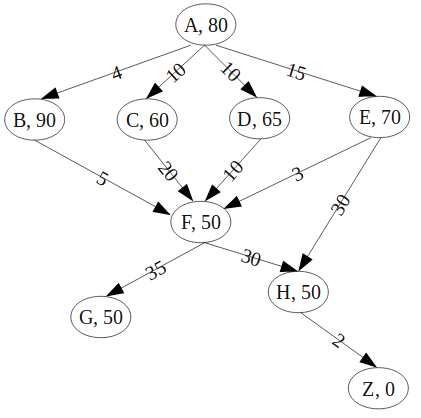
\includegraphics[scale=0.8]{grafo.png}\\
\raggedright
\vspace{1cm}
cerrada=NULL\\
abierta=A(0,80,80)\\
--------------\\
cerrada=A(0,80,80)\\
abierta=AB(4,90,94), AC(10,60,70), AD(10,65,75), AE(15,70,85)\\
--------------\\
cerrada=A(0,80,80), AC(10,60,70)\\
abierta=ACF(18,50,68), AB(4,90,94), AD(10,65,75), AE(15,70,85)\\
--------------\\
cerrada=A(0,80,80), AC(10,60,70), ACF(18,50,68)\\
abierta=ACFG(53,50,103), ACFH(50,50,100), AB(4,90,94), AD(10,65,75), AE(15,70,85)\\
--------------\\
cerrada=A(0,80,80), AC(10,60,70), ACF(18,50,68), AD(10,65,75)\\
abierta=ADF(20,50,70), ACFG(53,50,103), ACFH(50,50,100), AB(4,90,94), AE(15,70,85)\\
--------------\\
cerrada=A(0,80,80), AC(10,60,70), ACF(18,50,68), AD(10,65,75), ADF(20,50,70)\\
abierta=ADFG(55,50,105), ADFH(50,50,100), ACFG(53,50,103), ACFH(50,50,100), AB(4,90,94), AE(15,70,85)\\
--------------\\
cerrada=A(0,80,80), AC(10,60,70), ACF(18,50,68), AD(10,65,75), ADF(20,50,70), AE(15,70,85)\\
abierta=AEF(18,50,68), ADFG(55,50,105), ADFG(55,50,105), ADFH(50,50,100), ACFG(53,50,103), ACFH(50,50,100), AB(4,90,94)\\
--------------\\
cerrada=A(0,80,80), AC(10,60,70), ACF(18,50,68), AD(10,65,75), ADF(20,50,70), AE(15,70,85), AEF(18,50,68)\\
abierta= ADFG(55,50,105), ADFG(55,50,105), ADFH(50,50,100), ACFG(53,50,103), ACFH(50,50,100), AB(4,90,94)\\
--------------\\
cerrada=A(0,80,80), AC(10,60,70), ACF(18,50,68), AD(10,65,75), ADF(20,50,70), AE(15,70,85), AEF(18,50,68)\\
abierta=ABF(9,50,59) ADFG(55,50,105), ADFG(55,50,105), ADFH(50,50,100), ACFG(53,50,103), ACFH(50,50,100), AB(4,90,94)\\
--------------\\
cerrada=A(0,80,80), AC(10,60,70), ACF(18,50,68), AD(10,65,75), ADF(20,50,70), AE(15,70,85), AEF(18,50,68), ABF(9,50,59)\\
abierta=ABFG(44,50,94), ABFH(39,50,89), ADFG(55,50,105), ADFG(55,50,105), ADFH(50,50,100), ACFG(53,50,103), ACFH(50,50,100), AB(4,90,94)\\
--------------\\
cerrada=A(0,80,80), AC(10,60,70), ACF(18,50,68), AD(10,65,75), ADF(20,50,70), AE(15,70,85), AEF(18,50,68), ABF(9,50,59), ABFH(39,50,89)\\
abierta=ADFGZ(57,0,57), ABFG(44,50,94), ADFG(55,50,105), ADFH(50,50,100), ACFG(53,50,103), ACFH(50,50,100), AB(4,90,94)\\
--------------\\
cerrada=A(0,80,80), AC(10,60,70), ACF(18,50,68), AD(10,65,75), ADF(20,50,70), AE(15,70,85), AEF(18,50,68), ABF(9,50,59), ABFH(39,50,89), ADFGZ(57,0,57)\\
abierta=ABFG(44,50,94), ADFG(55,50,105), ADFH(50,50,100), ACFG(53,50,103), ACFH(50,50,100), AB(4,90,94)\\
\vspace{1cm}
La solución es ADFGZ
\pagebreak
\section{Ejercicio 2}
\subsection{Enunciado}
Apliques 10 pasos de A* sobre el problema 8-puzzle de la Figura 4.7 del libro "Artificial Intelligence. A Modern Approach", Segunda Edición, de Stuart Russel y Peter Norvig, con A* y la distancia de Manhatann como función heurística. Para este ejercicio, te sugiero que dibujes los estados que se generan, con enlaces entre estados padre y estados hijos, y que junto a cada estado pongas entre paréntesis la siguiente información
\begin{enumerate}
	\item Iteración en la que se generó el estado
	\item Nombre del estado (inventado)
	\item Coste del estado
	\item Valor heurístico del estado
	\item Suma del coste y del valor heurístico del estado
	\item Nombre del mejor padre.
\end{enumerate}

% \vspace*{\fill}
% \raggedleft Documento escrito en \LaTeX{}
\end{document}
